%% LyX 1.3 created this file.  For more info, see http://www.lyx.org/.
%% Do not edit unless you really know what you are doing.
\documentclass[english]{article}
\usepackage[T1]{fontenc}
\usepackage[latin1]{inputenc}
\usepackage{geometry}
\geometry{verbose,letterpaper,tmargin=1in,bmargin=1in,lmargin=1in,rmargin=1in}
\usepackage{subfigure}
\usepackage{graphicx}

\makeatletter

%%%%%%%%%%%%%%%%%%%%%%%%%%%%%% LyX specific LaTeX commands.
%% Bold symbol macro for standard LaTeX users
\providecommand{\boldsymbol}[1]{\mbox{\boldmath $#1$}}


\usepackage{babel}
\makeatother
\begin{document}

\title{Implementing the SynthBuilder Piano in STK}


\author{Stephen Sinclair}

\maketitle
{\begin{center}Final Project MUMT 614, Winter 2006\\McGill University\end{center}}




\section{Introduction}

In my project proposal, I suggested that it would be beneficial to
retrieve some of the work done by Stanford University's CCRMA group
in the early- to mid-1990's on the NeXT-based SynthBuilder project,
created by Staccato Systems. SynthBuilder was a graphical system for
physical modelling in which a user could make use of a variety of
so-called Unit Generators, filters, and other signal processing and
control parameter objects organized into a graph called a \emph{patch},
which would then generate code to be downloaded to the system's dedicated
DSP facilities, to run the algorithm in realtime. At the time, this
was the only way of achieving realtime performance, since general-purpose
processors were not fast enough to do so.

Some interesting models of various string instruments, electric guitars,
drums, and bells were created, often using innovative commuted synthesis,
modal synthesis, and waveguide techniques. However, SynthBuilder itself
depended on a module of the NeXTStep operating system called MusicKit,
and utilized many specific features of the Objective-C-based system
facilities for operation and file storage. Though this likely speeded
development and made for efficient code, it also made it difficult
to port the software to other systems, and so when NeXT became obsolete,
many of these SynthBuilder patches were effectively lost. Despite
the similarities between NeXTStep and Apple's modern OS X, SynthBuilder
has never been ported. In my personal opinion, this would still be
a worthwhile effort, but quite difficult, as it would also imply porting
all of MusicKit and re-writing large portions of both the back- and
front-ends.

However, now that computers are able to perform realtime synthesis,
many new DSP environments have been created. One of these is the Synthesis
Toolkit in C++ (STK), developed by Perry Cook of Princeton and Gary
Scavone of McGill University. STK is a good choice for building portable
applications because it is written in pure C++ and embeds a cross-platform
realtime audio and MIDI solution called RtAudio and RtMidi, respectively.
It is also free and open-source, placed in the public domain.


\section{Patches}

Two NeXT cubes were on-hand for running SynthBuilder, which fortunately
was still availabe on the Stanford web site. On running it, a {}``demo''
notice was displayed saying that some functionality would be disabled,
but enough functionality was available to be able to load and explore
the patches. Unfortunately, most would not actually run, as the machines
we had did not have the required DSP capabilities.

First, an attempt was made to read the SynthBuilder file format and
explore the possibility of writing a conversion software. However,
this proved easier said than done. SynthBuilder files were written
using the {}``Typed Stream'' format, an object serializing system
in the NeXT operating system. As such, the files consist of a binary-encoded
stream of class instances, of which some belong to SynthBuilder, some
to MusicKit, and some to NeXTStep. Although some source code for SynthBuilder
was available, the file format itself is not described fully by this
code. I created a Python-based parser that could read some information
from the files, but it was not successfully able to parse the entire
file format. It was decided that it would be a better use of time
and effort to use the SynthBuilder patches as reference for re-implementation
directly using STK classes as the processing units.

I chose to start with the Piano patch, as it was a fairly complete
example of synthesis techniques, including commuted synthesis, a two-string
coupled delay-line feedback loop, a modal synthesis algorithm for
the higher piano keys, and non-linear look-up tables for pre-computed
data.


\section{Piano}

The piano patch is presumed to be based on much of the findings in
\cite{smith_icmc95}. It is divided into three sections: the so-called
``piano driver'', which interprets incoming MIDI data and forwards it to
the correct algorithm (contained in subpatches), the {}``regular notes''
model, which contains the coupled string algorithm, and the {}``high
notes'' model, which uses a series of biquad (2$^{\textrm{nd}}$-order
IIR) filters with poles near the unit circle, causing them to ring
at particular resonant frequencies which are tuned to simulate a piano
note. Each of these resonant frequencies can be considered a mode
of vibration for the piano strings.

I began by taking screen shots of each subpatch, using NeXTStep's
Grab utility. You can view them in the appendix of this document.
The piano driver section mainly consisted of look-up tables containing
parameters for various objects in the synthesis algorithms. Using
TextEdit, it was possible to copy and paste these look-up tables into
a text file, which I then converted into C arrays.

The subpatches themselves were essentially block diagrams of the respective
synthesis algorithm. This made it quite straight-forward to implement
them by instantiating similar objects in STK. However, they also each
contained a reference to some C code. This code could be called by
the SynthBuilder patch through an Objective-C callback wrapper. It
was in this C code that the calculations were performed for the various
filter coefficients in each model.

\section{Regular Notes}

\begin{figure}[h]
\begin{center}
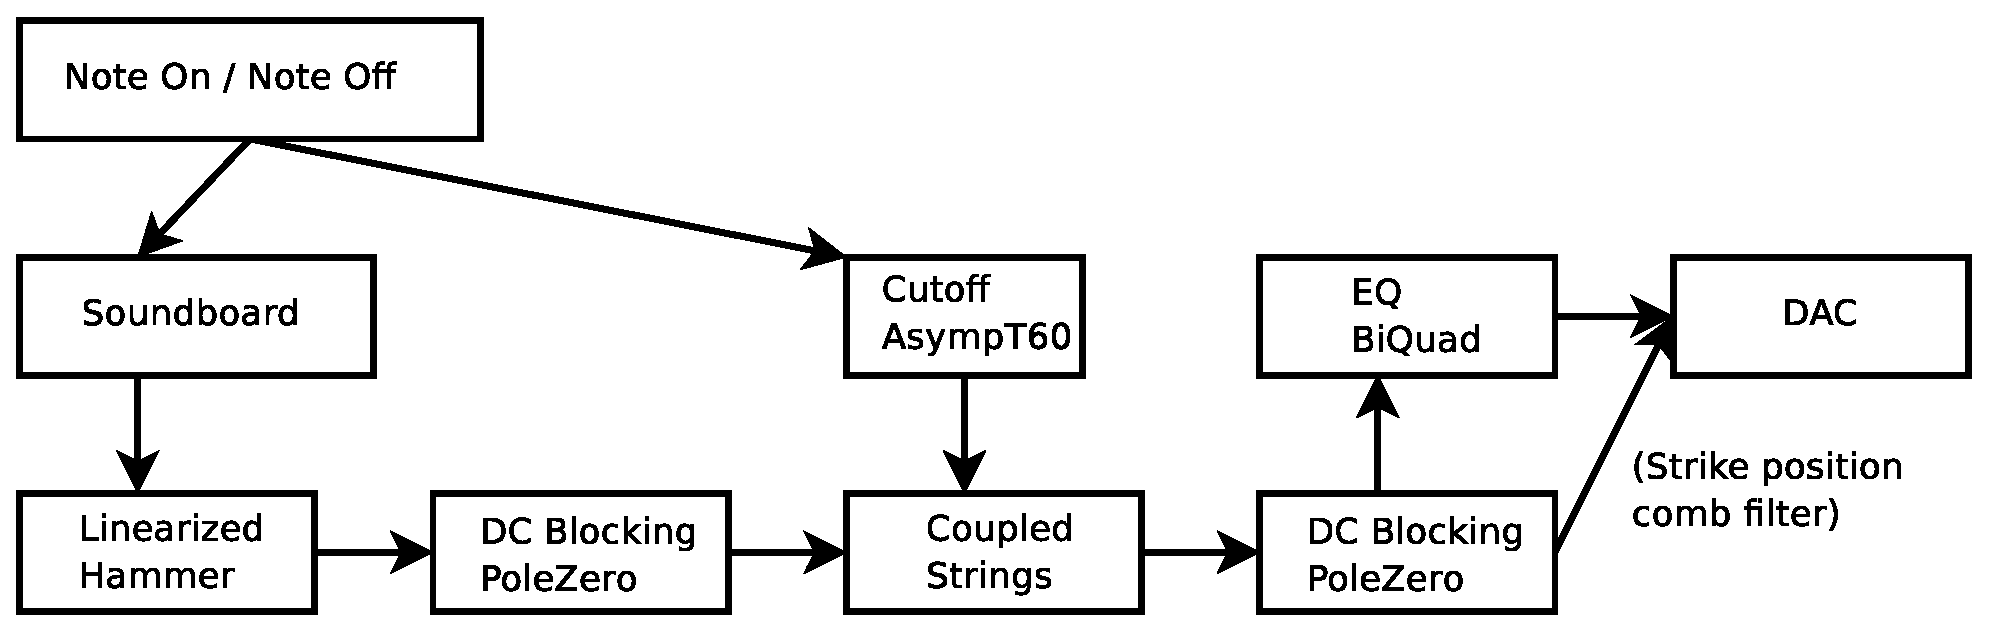
\includegraphics[width=5in]{regularmodel.eps}
\end{center}
\caption{Regular notes model}
\label{fig:regularnotes}
\end{figure}

The regular notes model, pictured in Figure~\ref{fig:regularnotes}, consists of
a soundboard model, a hammer model, and a coupled strings model.  The piano
has 2 strings, slightly detuned from one another.  The soundboard and
linearized hammer are commuted to the beginning of the whole piano model,
so that they can be used as inputs to the coupled string system instead
of being convolved with the ouptut.  This is an example of commuted
synthesis as described in \cite{smith_icmc95}.

The soundboard consists of a white noise source multiplied by two
exponentially decaying curves, one to model a ``tap'' on the soundbard,
the other to model the pedal. They are added, and the pedal envelope
does not start to decay until a ``note off'' message is received. This
simulates the pedal allowing the soundboard to resonate. Note that
there is mention in the code of a ``pedal filter'', which I did not
implement, as I could not find it in the patch.

The hammer is modeled by four low-pass OnePole filters in series. (See Figure~
\ref{fig:hammer} in the appendix.) These filters
simulate the felt on a piano hammer, which would dampen the high frequencies
in an otherwise dry impulse.  Two look-up tables, indexed according to note
number, contain pole values for ``loud'' and ``soft'' taps, with soft taps
having poles closer to the unit circle, thus cutting high frequencies to a
greater degree.  These two pole values are interpolated using a
``velocity warping'' table (called $normalizedVelocity$), which essentially
stretches the input velocity along
a kind of exponential curve.  This greatly increases the apparent effect of
amplitude response when hitting the keys of a velocity-sensitive MIDI keyboard.

The code for this velocity warping function is as follows:

\begin{quote}
\texttt{hammerPole = softPole + (loudPole - softPole)*normalizedVelocity}

\texttt{hammerGain = overallGain * (softGain + (loudGain -
softGain)*normalizedVelocity)}
\end{quote}

where \texttt{softPole} is in the range [0.95, 0.99] and \texttt{loudPole}
is in the range [0.84, 0.88].  \texttt{loudPole} itself can also be
adjusted by an exteral ``brightness'' value, in the range [-0.25, 0].
The transfer function can then be calculated as,

\begin{eqnarray*}
H(z) = \frac{(1-hammerPole)hammerGain}{1+(1-hammerPole)z^{-1}}
\end{eqnarray*}

This results in various degrees of low-pass behaviour depending on
which key was hit, and how hard.  (Here, \texttt{overallGain} can be
considered a ``loudness'' setting, where it is typically $\geq 1$.)

Examining the hammer analysis given in \cite{vanduyne_icmc95}, we see that
this hammer model does not incorporate the multi-pulse effect describe
there.  However, it does implement the non-linear felt response
(Section 2.2), described as being ``fundamentally a lowpass filter and a
DC-blocker''. The DC-blocker portion is assumed to refer to the PoleZero
filter found in the main ``regular model'' subpatch.

The coupled strings model feeds the filtered tap into two feedback delay
lines.  The delay line lengths are calculated to correspond to the
desired frequencies.  Each delay line has one all-pass to allow for
fractional delay, which I replaced with the STK DelayA class. Also
present is a series of 3 all-passes used to simulate string stiffness.
They are uniformly configured with the following transfer function:

\begin{eqnarray*}
H(z) = \frac{S_k k_s+z^{-1}}{1+{S_k k_s}z^{-1}}
\end{eqnarray*}

where $S_k$ is the ``stiffness coefficient'' found in a pre-computed look-up
table indexed by the note number, and $k_s$ is the adjustable ``stiffness
factor'', where $1 \leq k_s \leq 3.7$.

The outputs of both delay line systems are added and fed into a
coupling filter which simulates the energy transmitted between the two
vibrating strings, before being fed back into the input of each
delay line. Here, the damper is also modeled by providing a ``loop gain'',
an exponential decay which multiplies the input to the coupling filter,
and does not start to decay until a ``note off'' message is received.

The coupling filter is calculated as,

\begin{eqnarray*}
g &=& 10^{D/(20\omega)}\\
\gamma &=& 3(1-b)-g(1-a)\\
H(z) &=& \frac{\frac{2(g(1-a)-(1-b))}{\gamma}
  + \frac{2(a(1-b)-gb(1-a))}{\gamma}z^{-1}}
{1+\frac{gb(1-a) - 3a(1-b)}{\gamma}z^{-1}}
\end{eqnarray*}

where $D$ is the decay rate, $\omega$ is the frequency, $g$ is the
amount of attenuation on each sample period, and $a$ and $b$ are pole
and zero values pre-calculated (or measured) for a {\em single string}. In the
implementation, these pole and zero values are indexed by note number.

This coupled strings model is exactly similar to the one found in
\cite{vanduyne_icmc95}, which describes derivation of the coupling filter
equation in terms of an impedance model, along with the reasoning behind
the ``single string'' approach. It also includes a reference to the
authors' previous research on stiffness all-pass filters.

It should be noted that a
typical piano has three strings for each note, rather than two. However two
strings still gives a good impression of detuned oscillations, and to allow
for polyphonic implementations, it is important to be conservative in this
regard. A third string may be interesting for future improvements.

The output of the coupled strings is passed through a DC-blocking filter
and an ``EQ'' BiQuad filter. Although it is not clear from the patch
that this EQ is intended to be used as a comb filter, the C code makes
reference to a ``strike position comb filter''. Since the EQ tuning is
clearly dependant on a ``strike position'' value, I tried adding the
output of this EQ to its input, creating a comb filter, which clearly
improved the sound of the system. As such, I decided to leave it even
though I was not sure of the original intention.

\section{High Notes}

\begin{figure}[h]
\begin{center}
\includegraphics[width=4in]{highnotes.eps}
\end{center}
\caption{High notes model}
\label{fig:highnotes}
\end{figure}

After MIDI note number 88, or E7, the previous model is no longer
adequate for modeling high frequencies. The reason is that the delay
line for these high notes becomes very short, and the effect of the
all-pass interpolation is more obvious. In the high frequencies, the
all-pass interpolation is less accurate, and the model sounds out of tune.

Instead, a modal synthesis technique is used.  The soundboard model
is almost identical, with the addition of a 6-db/octave high-pass
OneZero filter. The hammer model is also similar, except that a
BiQuad filter is placed  after each of the 4 hammer filters. Each of
these BiQuads, pictured in Figure~\ref{fig:highnotes}, models a single
mode of vibration for the piano string.

Again, BiQuads are tuned using C routines. The tuning involves both the
positioning of the resonant mode and the setting of a gain factor.
Although the C code called for a gain of 1 on each of these BiQuads,
there also existed in the patch a look-up table called \texttt{bq4\_gEarBalled}
which was not referenced by the code. Immediately it was quite obvious
that the high notes were much louder (and sightly distorted). It seemed
that \texttt{bq4\_gEarBalled} was intended for the gain of the first BiQuad.
(They were numbered in a random order.)  Using this value (indexed by note
number), the results were much smoother. There was still an obvious difference
in amplitude between the regular model and the high notes model (heard by
hitting D7 and then E7 in sequence), so in an ad-hoc manner I attempted to
distribute this gain over the other BiQuads. It seemed best if the
\texttt{bq4\_gEarBalled} value was divided by two and distributed to the
first two BiQuads. A trial-and-error technique was regrettable here, but
somewhat unavoidable. With the gains tuned correctly, the two models
became indistinguishable.

For tuning the resonances of the BiQuads, the usual polar-coordinates
formula was used. This could have been replaced with a call to
\texttt{BiQuad::setResonance()}, but I decided to leave the original
code in place.

\begin{eqnarray*}
H(z) = \frac{1}{1 -2r_p\cos(2\pi\theta k_p)z^{-1}+ {r_p}^2z^{-2}}
\end{eqnarray*}

Where $k_p$ is the partial number.  In fact, $k_p$ is not exactly an integer.
Values slightly larger than the exact partial number were used, to create
a stretched tuning. First the third partial is created, followed by the
second, and then the first.  The reason for dividing the first partial
into two stages is not entirely clear to me, but possibly has to do with
the fact that it is supposed to be modeling two coupled strings. One of
these two filters is also given an active FIR numerator, making its transfer
function,

\begin{eqnarray*}
H(z) = \frac{
1 -2(e r_{11}+r_{12}(1-e))(\cos(2\pi\theta k_1)))z^{-1}
  + ( e {r_{11}}^2+(1-e){r_{12}}^2)z^{-2}}
{1 -2{r_{11}}\cos(2\pi\theta k_1)z^{-1}+ {r_{11}}^2z^{-2}}
\end{eqnarray*}

where the two radii, $r_{11}$ and $r_{12}$ are almost, but not quite, the
same, and $e$ is a look-up value called the ``second stage amp ratio''.
This ratio varies only from -30 dB to -30.633 dB, from note number 88 to 107.
(Part of the reason it is not clear is that the two stages use the same
$\theta$ value, whereas I would expect that two detuned strings should have
slightly differing $\theta$. However, I won't argue, because it sounds very
decent, with virtually no perceptual cues that the model has changed.)

\bibliographystyle{plain}
\bibliography{piano}

\appendix

\section{Appendix: Screenshots}

\begin{figure}[h]
\begin{center}
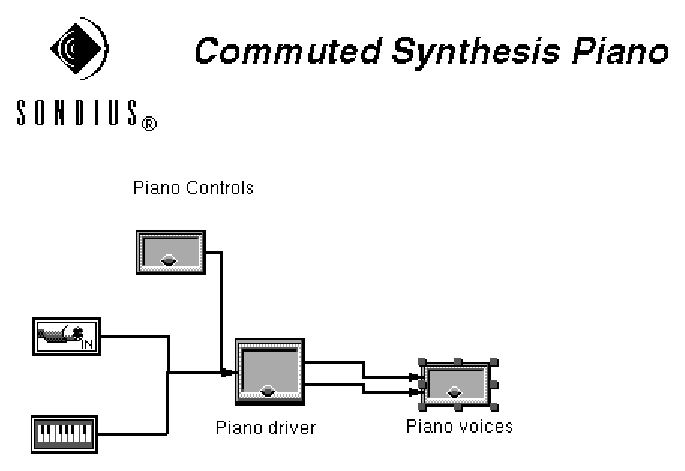
\includegraphics{../subpatches/mainpatch.eps}
\end{center}
\caption{Main piano patch}
\label{fig:mainpatch}
\end{figure}

\begin{figure}[h]
\begin{center}
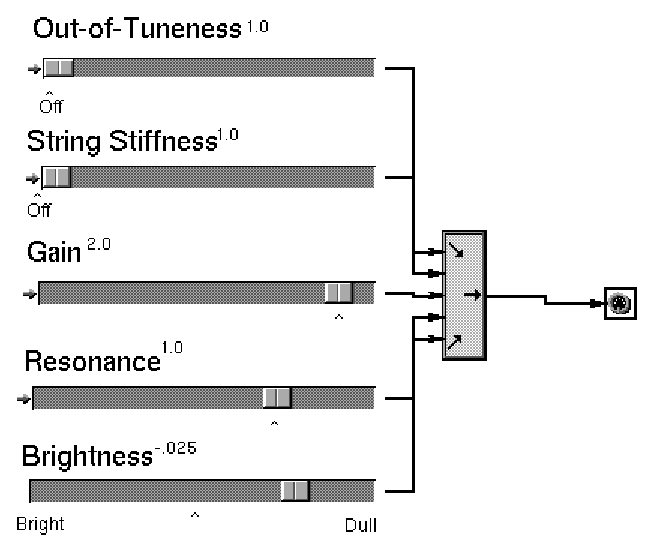
\includegraphics{../subpatches/controls.eps}
\end{center}
\caption{Controls. The only one that is inactive is Resonance, as it refers to
something called ``Pedal Presence Factor'' which is not referenced in the actual
DSP routine. There is reference to a ``pedal filter'' in the code, which I could not
find. I presume it was not fully implemented.)}
\label{fig:controls}
\end{figure}

\begin{figure}[h]
\begin{center}
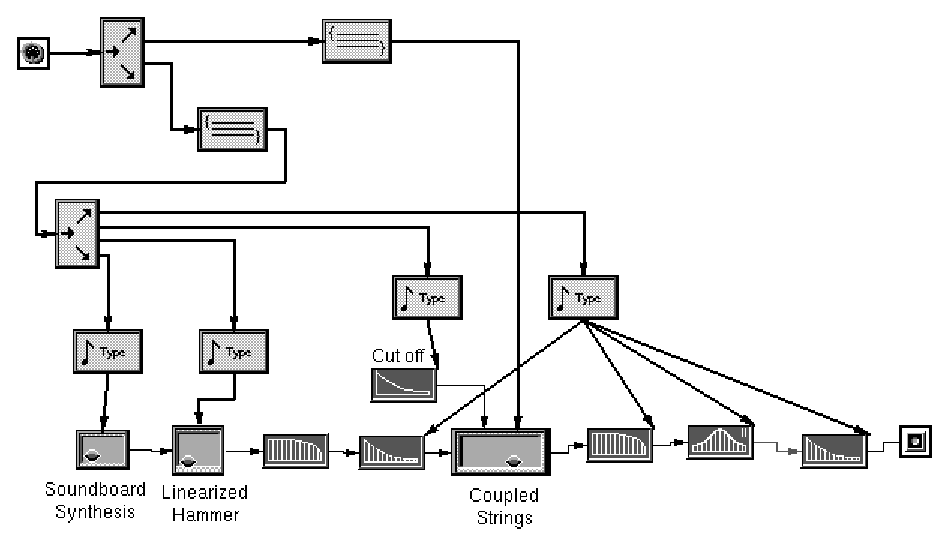
\includegraphics{../subpatches/regular.eps}
\end{center}
\caption{The regular notes model.}
\label{fig:regular}
\end{figure}

\begin{figure}[h]
\begin{center}
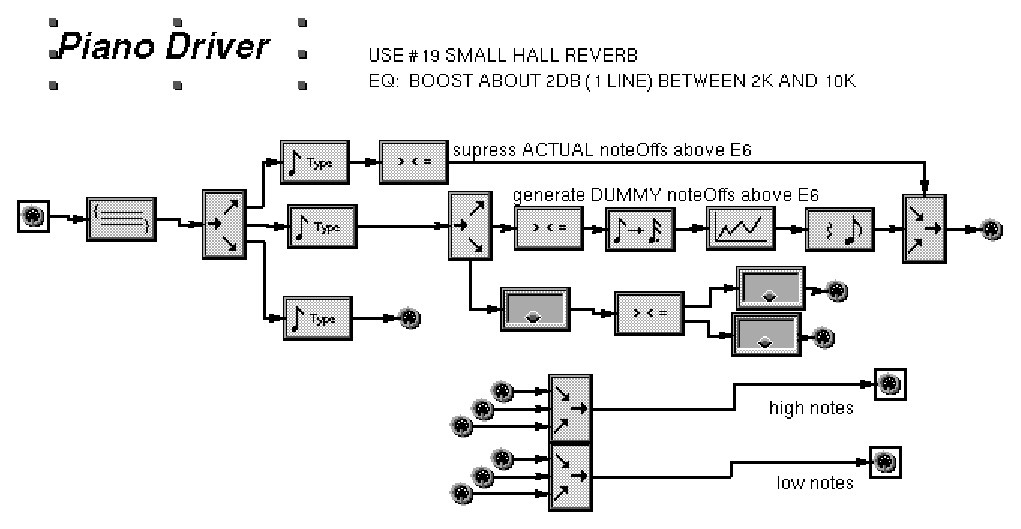
\includegraphics{../subpatches/pianodriver.eps}
\end{center}
\caption{The ``piano driver'' system, responsible for passing MIDI and control
data to the various subpatches.}
\label{fig:soundboard}
\end{figure}

\begin{figure}[h]
\begin{center}
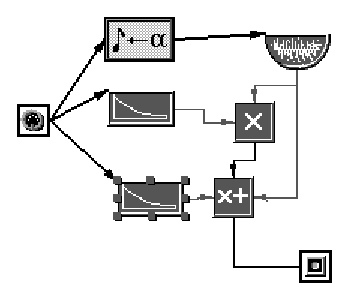
\includegraphics{../subpatches/soundboard.eps}
\end{center}
\caption{The soundboard model.}
\label{fig:soundboard}
\end{figure}

\begin{figure}[h]
\begin{center}
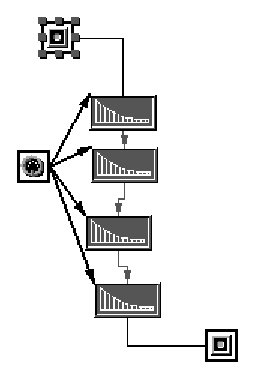
\includegraphics{../subpatches/hammer.eps}
\end{center}
\caption{The linearized hammer model.}
\label{fig:hammer}
\end{figure}

\begin{figure}[h]
\begin{center}
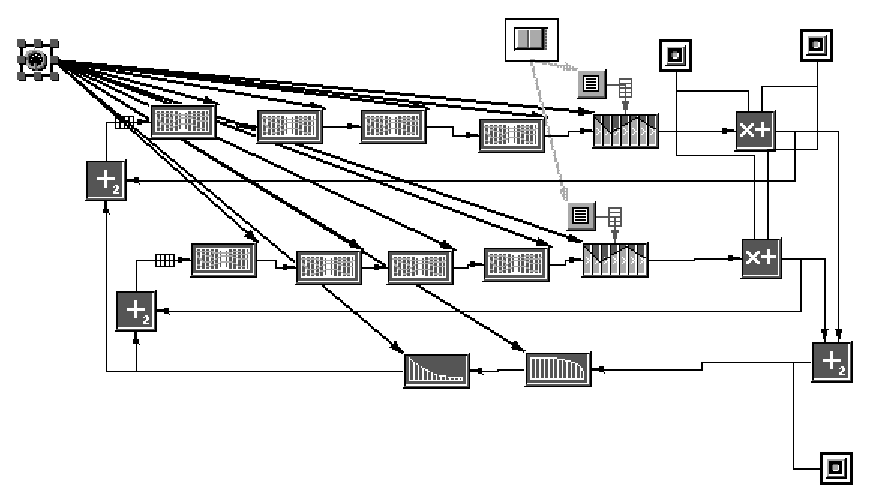
\includegraphics{../subpatches/coupledstrings.eps}
\end{center}
\caption{The coupled strings model.}
\label{fig:hammer}
\end{figure}

\begin{figure}[h]
\begin{center}
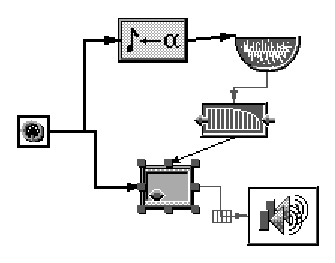
\includegraphics{../subpatches/highnotes_sb.eps}
\end{center}
\caption{The high notes soundboard model.}
\label{fig:hammer}
\end{figure}

\begin{figure}[h]
\begin{center}
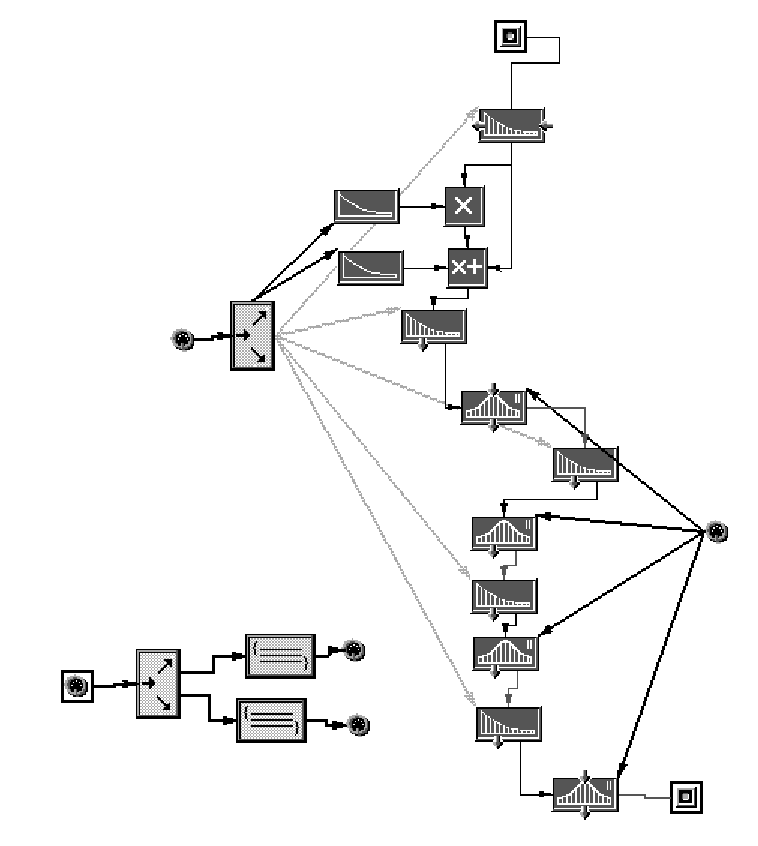
\includegraphics{../subpatches/highnotes_bq.eps}
\end{center}
\caption{The high notes hammer and BiQuad modal resonance model.}
\label{fig:hammer}
\end{figure}


\end{document}
